\documentclass[]{standalone}

\usepackage{amsmath}
\usepackage{amsfonts}
\usepackage{amssymb}
\usepackage{graphicx}
\usepackage{tikz}
\usepackage{import}
\usepackage[subpreambles=true]{standalone}

\usepackage{tikz}
\usepackage{tikz-3dplot}

\usetikzlibrary{positioning}
\begin{document}

    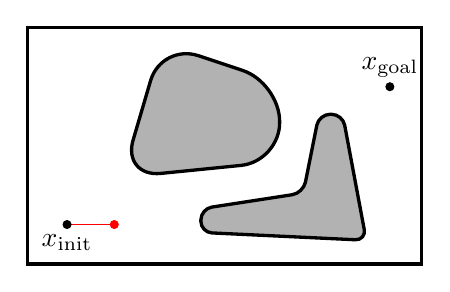
\begin{tikzpicture}[scale=1]

        \useasboundingbox (0,0) rectangle (5,3);

        \coordinate (init) at (0.5,0.5);
        \coordinate (goal) at (4.6,2.25);
        \coordinate (obs1) at (2.4,2.1);
        \coordinate (obs2) at (3.7,0.65);

        \coordinate (n0) at ($(init)+(0:0.6cm)$);
        \coordinate (n1) at ($(goal)!0.6cm!(n0)$);
        \coordinate (sample0) at (2, 1.8);
        \coordinate (n2) at ($(n1)!0.6cm!(sample0)$);
        \coordinate (n3) at ($(n0)!0.6cm!(n2)$);
        \coordinate (n4) at ($(n0)!1.2cm!(n2)$);
        \coordinate (sample1) at (3.5,0.3);
        \coordinate (n5) at ($(n4)!0.6cm!(sample1)$);
        \coordinate (n6) at ($(n2)!0.6cm!(n5)$);
        \coordinate (n7) at ($(n2)!1.2cm!(n5)$);

        % \coordinate (sample) at (0.8, 1.1);
        % \coordinate (sample_projection) at ($(init)!(sample)!(n0)$);
        
        \path[draw, very thick] (0,0) -- (5,0) -- (5,3) -- (0,3) -- cycle;
    
        \path[draw, red] (init) -- (n0);

        \path[draw, fill] (init) circle (0.05) node[below] {$x_\mathrm{init}$};
        \path[draw, fill] (goal) circle (0.05) node[above] {$x_\mathrm{goal}$};


        % \draw[draw, red] (sample_projection) -- (sample);
        
        % \foreach \x in {0,...,3}
        %     \path[draw, fill] (n\x) circle (0.05);

        \draw[draw, fill, red] (n0) circle (0.05);

        \path[draw, very thick, rounded corners=14pt, fill=black!30] (obs1) ++(-1.2,-1) -- ++(2,0.2) -- ++(0,1) -- ++(-1.5,0.5) -- cycle;
        \path[draw, very thick, rounded corners=4pt, fill=black!30] (obs2) ++(-1.5,-0.25) -- ++(0,0.3) -- ++(1.3,0.2) -- ++(0.2,1) -- ++(0.3,0) -- ++(0.3,-1.6) -- cycle;

    \end{tikzpicture}
\end{document}